\documentclass[12pt]{article}
\usepackage{ucs}
\usepackage[utf8x]{inputenc}
\usepackage[russian]{babel} 
\usepackage{amssymb}
\usepackage{amsmath}
\usepackage{mathtools}
\usepackage{tabularx}

\usepackage{geometry}
\geometry{left=2cm}
\geometry{right=2cm}
\geometry{bottom=2cm}
\geometry{top=2cm}

\usepackage{tikz}
\usetikzlibrary{arrows,automata}

\usepackage{xcolor}

\newcommand\tab[1][1cm]{\hspace*{#1}}

\begin{document}
\begin{titlepage}
\newpage
\begin{center}
Санкт-Петербургский государственный университет \linebreak Математико-механический факультет\\
\vspace{2cm}
КРАВЧЕНКО ЕВГЕНИЙ АРТУРОВИЧ\\
\vspace{1cm}
РЕФЕРАТ\\
\textsc{\textbf{СИНТЕЗ РАСПОЗНАВАТЕЛЯ КСР-ЯЗЫКА\\ ПО СИНТАКСИЧЕСКОЙ ГРАФ-СХЕМЕ}}\\
\vspace{2cm}
Математическое обеспечение и администрирование\\ информационных систем\\
\vspace{3cm}
Группа №344\\
\vspace{2cm}
Санкт-Петербург 2017
\end{center}
\end{titlepage}

\section{Введение}
На сегодняшний день область применимости языковых технологий очень велика. Они активно используются в различных сферах нашей жизни, что привело к созданию множества различных программ для обработки данных, использующих принципы синтаксического анализа.\\

Опыт построения систем для автоматического построения трансляторов показывает, что их удобно задавать с помощью КСР(КС грамматики в регулярной форме) грамматик. Процесс анализа при этом проводится с помощью магазинного автомата. На каждой итерации программа анализа обращается к управляющей таблице этого автомата для определения следующего состояния. Такой автомат можно построить по синтаксической граф-схеме КСР языка. Регулярное представление правил грамматики позволяет представить их в виде ориентированных графов. На их основе строятся состояния автомата.\\

В данной работе рассматривается алгоритм построения состояний распознавателя КСР-языка и его реализация. 
\section{Постановка задачи}
Задача - по заданной КСР-грамматике построить КСР-распознаватель, проверяющий входняе цепочки символов на принадлежность КСР-языку, порождаемому этой грамматикой. При этом на КСР-грамматику накладывается ограничение в виде отсутствия левой рекурсии.
\section{Описание и структура программы}
Программа состоит из трех этапов:
\begin{enumerate}
\item По КСР-грамматике построить эквивалентную ей линейную граф-схкму
	\begin{enumerate}
		\item[a] Закодировать входную грамматику
		\item[b] Полученную последовательность чисел преобразовать в граф-схему
	\end{enumerate}
\item По граф-схеме построить состояния КСР-распознавателя
	\begin{enumerate}
		\item[a] Сгенерировать множество состояний
		\item[b] Удалить эквивалентные состояния
	\end{enumerate}
\item Построить распознаватель
\end{enumerate}

\section{Представление данных}
\tab Программа принимает текствый файл, содержащий запись КСР-грамматики в виде последовательности $"N : r(A)."$, где $N$ - нетерминал, $r(A)$ - некоторое обобщенно-регулярное выражение. При этом первый нетерминал считается начальным. Файл должен заканчиваться строкой $"Eogram."$.\\

Синтакстическая граф-схема - это графовый аналог правил КСР-грамматики. Ее приедстваление в виде одномерного массива называется линейной граф-схемой.
Таким образом, линейная граф-схема - это представление КСР-грамматики в виде последовательности символов-команд $"↓,\ <,\ *,\ .\ "$, адресов перехода и терминалов.\\

Состояние - элемент одного из следующих видов: 
\begin{enumerate}
\item[a.] $\{ a - n \}$, где a - терминал, n - номер правила
\item[b.] $\{ F \}$ - конечное состояние
\item[с.] $\{ s_1, s_2, s_3, ... s_n\}$, где $s_i$ - состояния
\item[d.] $( s, N - n )$, где $s$ - состояние, $N$ - нетерминал, $n$ - номер правила
\end{enumerate}
\section{КСР-грамматика}
КС грамматика в регулярной ворме - это КС грамматика, в которой правые части правил представлены в виде обобщенно-регулярных выражений над символами объединенного алфавита грамматики.\\

Изначально грамматика представлена в виде последовательности лексем, однако для программы такое представление неудобно, поэтому первый шаг программы - кодирование КСР грамматики. Программа считывает правила (каждое из которых начинается с нетерминала и двоеточия, а оканчивается точкой) до тех пор, пока не встретит $"Eogram."$. Затем каждое правило разбивается на отдельные лексемы - нетерминалы и терминалы. Каждой лексеме присваивается уникальный номер(код) и она добавляется в кодировочную таблицу. Последним действием все лексемы заменяются на свои коды.
\section{Граф-схема}
Второй шаг - построение граф-схемы. Для этого каждое из каждого закодированного правила извлекается нетерминал и соответствующее ему регулярное выражение. По последнему строится(1) линейное представление его синтаксической граф-схемы. Построение проходит по следующим правилам:\\
\begin{center}
\begin{tabular}{|c|c|c|}
	\hline
	\texttt{a} & \texttt{->} & \texttt{a}\\\hline
	 \texttt{( A )} &\texttt{->}& \texttt{A}\\\hline
	 \texttt{A ; B}&\texttt{->} &\texttt{< \ n\  \ A \ ↓ \ m \ B}\\\hline
  $\texttt{[ A ]}$ & \texttt{->} &\texttt{ <\ n\ A}\\\hline
	\texttt{A*}&\texttt{->} &\texttt{ <\ n\ A \ ↓\ m}\\\hline
	 \texttt{A\#B} &\texttt{->}&\texttt{ A (B;A)*}\\\hline
	\texttt{(A\#)}&\texttt{->}&\texttt{ A*}\\\hline
	 \texttt{(\#A)}&\texttt{->}&\texttt{A A}\\\hline
	 \texttt{(;A)}&\texttt{->}&\texttt{ < \ n \ A}\\\hline
	\texttt{(A;)}&\texttt{->}&\texttt{ (;A)}\\\hline
	 \texttt{N} &\texttt{->}&\texttt{* \ N}\\\hline

\end{tabular}\\
\end{center}
	\tab Здесь $a$ - произвольный терминал (его закодированное представление),$N$ - нетерминал (его код), $A,B$ - регулярные выражения. $m$ и $n$ - адреса переходов.\\
	
Полученная последовательность записывается в виде массива целых чисел (символы $" ↓, <, *, ."$ также имеют кодовое представление) и сопоставляется с соответствующим нетерминалом. Затем к массиву соответствующему начальному нетерминалу "приписываются" все остальные, при этом для каждого нетерминала $N^i$ запоминается номер первого этемента соответствующего ему массива $N^i_{pos}$ в полученном массиве (2). Для того, чтобы полученный массив стал линейной граф-схемой, осталось заменить все коды нетерминалов $N^i$ на номера $N^i_{pos}$ (3). \\

Пример (для наглядности, без кодировки):\\
$\tab \texttt{Firts  : 'Hello', Second, ('!'; '!!!').}\\
\tab \texttt{Second : 'World'.}\\
\tab \texttt{Eogram.}
$
\\

После (1):\\
\tab\begin{tabular}{|c|c|c|c|c|c|c|c|c|c|c|c|}
\hline
\ & \ & \texttt{0} & \texttt{1} & \texttt{2} & \texttt{3} & \texttt{4} & \texttt{5} & \texttt{6} & \texttt{7} & \texttt{8} & \texttt{9}\\
\hline
\texttt{First} & \ & \texttt{'Hello'} & \texttt{*} & \texttt{Second} & \texttt{<} & \texttt{8} & \texttt{'!'} & \texttt{↓} & \texttt{9} & \texttt{'!!!'} & \texttt{.}\\
\hline
\texttt{Second} & \ & \texttt{'World'} & \texttt{.} & \ & \ & \ & \ & \ & \ & \ & \ \\
\hline
\end{tabular}
\\

После (2):\\
\tab\begin{tabular}{|c|c|c|c|c|c|c|c|c|c|c|c|}
\hline
\texttt{0} & \texttt{1} & \texttt{2} & \texttt{3} & \texttt{4} & \texttt{5} & \texttt{6} & \texttt{7} & \texttt{8} & \texttt{9} & \texttt{10} & \texttt{11}\\
\hline
\texttt{'Hello'} & \texttt{*} & \texttt{Second} & \texttt{<} & \texttt{8} & \texttt{'!'} & \texttt{↓} & \texttt{9} & \texttt{'!!!'} & \texttt{.} & \texttt{'World'} & \texttt{.}\\
\hline
\end{tabular}\quad \texttt{;} \quad
\begin{tabular}{|c|c|}
\hline
\texttt{$N^i$} & \texttt{$N^i_{pos}$}\\
\hline
\texttt{First} & \texttt{0}\\
\hline
\texttt{Second} & \texttt{10}\\
\hline
\end{tabular}
\\

После (3):\\
\tab\begin{tabular}{|c|c|c|c|c|c|c|c|c|c|c|c|}
\hline
\texttt{0} & \texttt{1} & \texttt{2} & \texttt{3} & \texttt{4} & \texttt{5} & \texttt{6} & \texttt{7} & \texttt{8} & \texttt{9} & \texttt{10} & \texttt{11}\\
\hline
\texttt{'Hello'} & \texttt{*} & \texttt{10} & \texttt{<} & \texttt{8} & \texttt{'!'} & \texttt{↓} & \texttt{9} & \texttt{'!!!'} & \texttt{.} & \texttt{'World'} & \texttt{.}\\
\hline
\end{tabular}
\section{Определение состояний в граф-схеме}
Следующий этап программы - построение состояний. \\
Состояния делятся на несколько видов:\\
\begin{enumerate}
\item[a.] $\{ a - n \}$ - если существует префикс непрочитанной части входной цепочки совпадающий с терминалом $a$, то можно прочитать этот префикс, перейдя в состояние $n$
\item[b.] $\{ F \}$ - конечное состояние, если цепочка прочитана полностью, а стек пуст, то цепочка принята, если стек не пуст, то вытолкнуть один элемент и использовать его в качестве номера следующего состояния
\item[с.] $\{ s_1, s_2, s_3, ... s_n\}$ - вектор состояний, можно перейти в любое из них
\item[d.] $( s, N - n )$ - можно перейти в состояние $s$, при этом в стек добавляется номер $n$ 
\end{enumerate}
Для построения используется следующая рекурсивная функция:\\
\\
\texttt{
\tab f(i):\\
\tab  \tab next := i + 1\\
\tab \tab if\ table[next].type == terminal\\
\tab  \tab \tab return \{ table[next] - next \}\\
\tab  \tab elif\ table[next].type == number\\
\tab  \tab \tab return f(table[next])\\
\tab  \tab elif\ table[next].type == *\\
\tab \tab \tab return ( f(next) , table[next] - next + 1 )\\
\tab  \tab elif\ table[next].type == <\\
\tab  \tab \tab return \{ f(next), f(next + 1) \}\\
\tab  \tab elif\ table[next].typ1e == ↓\\
\tab  \tab \tab return f(next)\\
\tab  \tab elif\ table[next].type == .\\
\tab  \tab \tab return \{ F \}\\
}

Данная функция кадой позиции в граф-схеме сопоставляет некоторое состояние, которое определяет, какие цепочки символов могут быть приняты в текущий момент. (Начальное состояние при $i = -1$)
\\

Рассмотрим пример:\\
$\tab \texttt{A  : 'a', B, 'c'.}\\
\tab \texttt{B : 'b'.}\\
\tab \texttt{Eogram.}
$\\

Линейная граф-схема:\\
\tab\begin{tabular}{|c|c|c|c|c|c|c|}
\hline
\texttt{0} & \texttt{1} & \texttt{2} & \texttt{3} & \texttt{4} & \texttt{5} & \texttt{6}\\
\hline
\texttt{'a'} & \texttt{*} & \texttt{5} & \texttt{'c'} & \texttt{.} & \texttt{'b'} & \texttt{.}\\
\hline
\end{tabular}\\

Применение функции $f$ даст следующий результат:\\
\texttt{
\tab f(-1) : \{ 'a' - 0 \}\\
\tab f(0)  : (\{ 'b' - 5 \}, B - 2)\\
\tab f(1)  : (\{ 'b' - 5 \}, B - 2)\\
\tab f(2)  : \{ 'c' - 3 \}\\
\tab f(3)  : \{ F \}\\
\tab f(4)  : \{ 'b' - 5 \}\\
\tab f(5)  : \{ F \}\\
}

Очевидно, что среди этих состояний ескть как эквивалентные, так и недостижимые. Для того чтобы определить эквивалентные состояния, используется хэш-суммы. После удаления дублей и недостижимых состояний, получим:\\
\texttt{
\tab S = \{ 'a' - 0 \}\\
\tab S0  = (\{ 'b' - 5 \}, B - 2)\\
\tab S2  = \{ 'c' - 5 \}\\
\tab S5  = \{ F \}\\
}

Для данного примера это минимальное количество состояний.

На данный момент состояния представляют собой цепочку вложенных друг в друга элементов различных классов. При анализе цепочки такое представление не удобно. Поэтому с полученными состояниями проводится еще одно преобразование : с помощью рекурсивного обхода строятся состояния вида $S_i\ /\ a = S_k\ [\ st_1 ... st_n\ ]$, где $S_i$ - состояние, $a$ - цепочка символов, $S_k$ - состояние, в которое попадет распознаватель при прочтении цепочки $а$, будучи в состоянии $S_i$. $st_1 ... st_n$ - числа которые при этом должны попасть на стек.
\\

Для приведенного выше примера результат будет следующим:\\  
\texttt{
\tab S / 'a' = S0 [ ]\\
\tab S0 / 'b' = S5 [2]\\
\tab S2 / 'c' = S5 [ ]\\
\tab S5 = F\\
}
\\

Для того, чтобы проверить строку на принадлежность грамматике, начнем проверять префиксы входной чепочки и применять соответствующие переходы. Для примера посмотрим на проверку строки $'abc'$ для построенных выше правил: \\
(начальное состояние - S, входная цепочка - 'abc', стек пуст)

\texttt{
( S, 'abc', [ ] ) $\xrightarrow{\texttt{a}}$ ( S0, 'bc', [ ] ) $\xrightarrow{\texttt{b}}$ ( S5, 'c', [2] ) $\xrightarrow{\texttt{pop( )}}$\\\tab ( S2, 'c', [ ] ) $\xrightarrow{\texttt{c}}$ ( S5, , [ ] ) $\xrightarrow{\texttt{pop( )}}$ ( , , [ ] )
}

Значит входная цепочка приинадлежит грамматике, поскольку при проверке распознаватель попал в конечное состояние, при котором не осталось непрочитанных символов и стек оказался пустым.
 
\section{Основные классы или функции в программе}
Программа написана на языке С++, ниже описаны основные функции и классы программы. (Если для какого-либо метода/функции нет описания, значит он является вспомогательным)\\
\\
Таблица для кодировки представлена в программе следующим образом:\\\\
\texttt{
class c\_Table\\
\{\\
\tab	vector<string> nonterms;\\
\tab	vector<string> terms;\\\\
public:\\
\tab	enum ct\_TYPE \{\\
\tab\tab		NONT = 0,\\
\tab\tab		TERM = 1\\
\tab	\};\\\\
\tab	c\_Table();\\\\
\tab	int get\_int(const string \& s);\\
\tab	string get\_string(int i);\\
\tab	int add(const string \& s, ct\_TYPE type);\\
\tab	ct\_TYPE getType(int i);\\\}
}

Элементы в таблице могут быть двух видов : терминалы и нетерминалы, которые хранятся в соответствующих массивах. \\
Функция $add$ позволяет добавить элемент $s$ с типом $type$ в таблицу и возвращает код, присвоенный этому элементу.\\
Функция $get\_int$ по элементу позвращает его код, $get\_string$ - наоборот.\\
$getType$ позвращает тип элемента по его коду.\\
\\

Кодировка проводится с помощью объекта следующего класса:
\\
\texttt{class c\_Encoder\\
\{\\
\tab	string getNxt(istream \& input);\\
\tab	string getNword(const string \& s, int \& n);\\
\tab	vector<int> enc(const string \& s);\\
\\
\tab	c\_Table table;\\
public:\\
\tab	vector< vector<int> > encoded;\\
\\
\tab	int getTint(const string \& s);\\
\tab	string getTstr(int i);\\
\tab	c\_Table::ct\_TYPE getType(int i);\\
\\
\tab	void Encode(istream \& input);\\
\}
}
\\

Тут $table$ - кодировочная таблица, $encoded$ - закодированное представление грамматики в виде двумерного массива.\\
Функция $Encode$ производит кодировку. В качестве параметра передается поток ввода, результат работы попадает в $table$ и $encoded$.
\\

Линейная граф-схема представлена следующим классом:\\
\\
\texttt{class lin\_Table\\
\{\\
\tab 	class element;\\
\\
\tab 	c\_Encoder encoder;\
\\
\tab 	void recgen(int i, int l, int r);\\
\tab 	void generate(int i);\\
\tab 	string elem\_to\_str(element e);\\
\tab 	unordered\_map<int, int> nonts;\\
\\
public:\\
\tab 	class element \{\\
\tab 	public:\\
\tab \tab 		enum elType \{\\
\tab \tab \tab 			NUM = 0,\\
\tab \tab \tab 			TERM = 1,\\
\tab \tab \tab 			NONT = 2,\\
\tab \tab \tab 			ARROW = 3,\\
\tab \tab \tab 			ASTER = 4,\\
\tab \tab \tab 			CASES = 5,\\
\tab \tab \tab 			DOT = 6\\
\tab \tab 		\};\\
\tab \tab 		elType t;\\
\tab \tab 		int val;\\
\tab \};\\
\\
\tab	vector<element> table;\\
\\
\tab 	int get\_Nont(int pos);\\
\tab 	string get\_FCTstr(int i);\\
\\	
\tab 	lin\_Table(istream \& input);\\
\tab 	void print(std::ostream \& out);\\
\}}
\\

Здесь $encoder$ - закодированная грамматика, $table$ - ее линейние представление, являющееся массивом элементов типа $element$. $element$ - это класс, у которого есть поля 'значениt'($val$) и 'тип'($t$). Тип определяет роль элемента в таблице, значение необходимо только для элементов типов $NUM,\ TERM,\ NONT$. \\
Преобразование в граф-схему выполняется внутри конструктора класса. Для этого необходимо передать поток ввода. При этом задействуются приватные рекурсивные функции класса, а также переменная $nonts$, которая позволяет выполнить преобразование (3) (см. пункт 6 Граф-схема).\\
$print$ печатает полученный массив в переданный поток вывода.
\\
\\

Следующие классы описывают состояния:
\begin{verbatim}
class Element_base {
public:
    virtual int getType() = 0;
    virtual void print(std::ostream & out, lin_Table & tbl) = 0;
    virtual long hash(tableType * t) = 0;
    virtual void update(samestates & m, tableType & t, bool * valid) = 0;
};

class Element_final : public Element_base {
public:
    Element_final() {};
    int getType();
    void print(std::ostream & out, lin_Table & tbl);
    long hash(tableType * t);
    void update(samestates & m, tableType & t, bool * valid) {}
};

class Element_simple : public Element_base {
public:
    int term, pos;
    long H;
    Element_simple(int t, int p);
    int getType();
    oid print(std::ostream & out, lin_Table & tbl);
    long hash(tableType * t);
};

class Element_vector : public Element_base {
public:
    long H;
    vector<shared_ptr<Element_base>> elements;
    Element_vector(shared_ptr<Element_base> e1, shared_ptr<Element_base> e2);
    int getType();
    void print(std::ostream & out, lin_Table & tbl);
    long hash(tableType * t);
    void update(samestates & m, tableType & t, bool * valid);
};

class Element_call : public Element_base {
public:
    int Nont, retpos;
    shared_ptr<Element_base> element;
    long H;
    Element_call(int n, int p, shared_ptr<Element_base> e);
    int getType();
    void print(std::ostream & out, lin_Table & tbl);
    long hash(tableType * t);
    void update(samestates & m, tableType & t, bool * valid);
};
\end{verbatim}

Как видно, тут в точности описаны все 4 типа состояний, причем все они наследуются от одного базового класса $Element\_base$. Каждый класс имеет метод для печати а поток - $print$, вычисления хэш-суммы - $hash$, а также обновления - $update$ (данный метод необходим при удалении дублей, он заменяет все указатели на элемениы с одинаковой хэш-суммой на один общий). Следует также отметить поле $H$. Это поле используется для того, чтобы не пересчитывать хэш-сумму каждый, что может быть довольно долгим процессом, так как функция $hash$ рекурсивно обходит все состояния. После того как хэш посчитан, он сохраняется в $H$, и при следующем вызове $hash$ будет просто возвращено это значение.\\\\ 

Определим следующие типы:\\
\texttt{
typedef unordered\_map<long, vector<int> > samestates;\\
typedef map< int, shared\_ptr< Element\_base > > states\_t;\\
typedef map< int, vector< pair< string, pair<int, vector<int> > > > > simple\_states;\\}Где $states\_t$ - тип состояния, $samestates$ - тип словаря, сопоставляющего хеш-сумме множество номеров состояний, $simple\_states$ - тип состояний для распознавателя.\\
\\

Следующий класс отвечает за построение состояний:\\
\texttt{
\\
class Analyzer\_states\{\\
\tab 	shared\_ptr<Element\_base> getState(lin\_Table \& tbl, tableType \& table, int pos);\\
\tab 	void simplify(int state, shared\_ptr<Element\_base> e, vector<int> \& st, lin\_Table \& table);\\
\\
public:\\
\tab 	states\_t States;\\
\tab 	simple\_states SS;\\
\\
\tab 	Analyzer\_states(lin\_Table \& tbl);\\
\tab 	void printStates(ostream \& out, lin\_Table \& t);\\
\\
\tab 	simple\_states get\_states(lin\_Table \& table);\\
\};}\\

Как и в $lin\_Table$, поздание состояний происходит в конструкторе. Сначала при помощи $getState$ генерируется и минимизируется множество состояний $States$, которое затем функцией $simplify$ преобразуется в множество состояний $SS$, которое непосредственно используются в распознавателе.\\
$get\_states$ возвращает состояния распознавателя, $printStates$ - печатает в поток вывода.
\\
\\

Сам распознаватель представлен в виде следующего класса:\\
\\
\texttt{class Analyzer\\
\{\\
\tab 	simple\_states states;\\
\tab 	int rec\_analyzer(const string \& str, int l, int state, vector<int> \& st);\\
\\
public:\\
\\
\tab 	int analyze(const string \& str);\\
\tab 	Analyzer(istream \& input){};\\
\}\\
}\\

В $states$ хранятся правила(пересходные состояния) распознавателя.\\
Метод $analyze$ проверяет строку на принадлежность грамматике(используя рекурсивную функцию $rec\_analyzer$). Если строка принята, то возвращается $INT\_MAX$, иначе позиция, на которой произошла ошибка.
\\

Таким одразом, для того, чтобы создать распознаватель КСР-грамматики из файла $grm.txt$, достаточно написать \\
\tab\texttt{Analyzer A(if`stream("grm.txt"));}\\
Проверить строку на принадлежность можно следующим образом:\\
\tab \texttt{int res = A.analyze("Hello, world!");}

\section{Результат}

\tab Программа реализована на языке С++ с использованием возможностей страндарта С++11. Также были использована библиотека \texttt{Windows.h} для взаимодействия с консолью ОС Windows. Вся программа разбита на 5 модулей. Суммарное количество строк исходного кода около 950. Размер исполняемого файла составляет 86Кб.\\

Сначала спрашивается имя файла с грамматикой. Затем способ ввода(с клавиатуры / из файла).\\
Программа работает в консольном режиме: строит распознаватель по входной КСР-грамматике, а затем проверет входные цепочки на принадлежность грамматике. При этом, если цепочка не принята, она разбивается на 2 части: префикс, который может являться началом цепочки данного КСР-языка и оставшаяся часть (которую распознаватель не принял). Обе части выводятся в консоль и при этом подсыечиваются различными цветами.



Посмотрим на работу распонавателя на примере грамматики Yard:
\begin{verbatim}
Program :(; 'static' ) , 'program' , '<tag>' , '(' , ( 'input' ; 'output' ; '<tag>' 
	)#( ',' ) , ')' , (#( ';' ,  Declaration)) , ';' , CompoundStatement , '.' .
ArraySpecification : 'array' , FormalBounds , FormalComponent ; '<tag>',(; 	
	FormalBounds ) , (; FormalComponent ) . 
CompoundStatement : 'begin',( NetExpression )#( ';' ) , 'end'  ; 'if' , 	
	NetExpression , 'then',( NetExpression)#( ';' ) , (; ('else' ,( NetExpression 
	)#(';' ) )) , 'endif' .
Constant : '<number>' ; '<real>' ; '<string>' ; '<char>' .
ConstantDeclaration : 'const' ,( '<tag>' , '=' , Operand )#( ';' ) .
Declaration : ConstantDeclaration ; VariableDeclaration ; NodeDeclaration .
FormalBounds : '[' , (; ( '<tag>' ; Constant ,(; '..' ,Constant ) )#( ',' ) )
	, ']'.
FormalComponent : 'of' , Specification .
ForStatement : 'for' , 'all' , '<tag>' , 'do' ,(  NetExpression ; 
	CompoundStatement ).
NetExpression : (#( '<operation>' ) , Operand , (; PrimitiveResource ) )#(
	'<operation>' ) ; Operand , (; PrimitiveResource ) , ':=' , NetExpression ;
 	ForStatement .
NodeDeclaration : 'node' , VariableDeclaration ; (; 'static' ) , 'node' , '<tag>' ,
	 (; ( '(' , ( '<tag>' )#( ',' ) ,')' ) ) ; CompoundStatement .
Operand : '<tag>' , (#( SliceConstructor ; '^' ) ) ; '(' , NetExpression , ')' ;
 	'<tag>' , (; '(' , ( '<tag>' )#( ',' ) , ')' ) ; Constant . 
PointerSpecification : 'pointer' ,(; ( (; 'to' ) , '<tag>' ) ) .
PrimitiveResource : '@' , ( 'input' ; 'output' ; '<tag>' ) .
SliceConstructor : '[' , ( SubscriptExpression )#( ',' ) , ']' .
Specification : ( 'bool' ; 'byte' ; 'char' ; 'dword' ; 'int' ; 'longint' ; 'shortint'
 	; 'word' ; 'bitrow' ; 'double' ; 'pointer' ; 'real' ; 'string' ),(;  '*' ,
  	'<number>' )  ; PointerSpecification ; ArraySpecification .
SubscriptExpression : '<tag>' ; 'all' ; NetExpression ; '(' , ( SubscriptExpression 
	)#( ',' ) , ')' .
VariableDeclaration : ( ( '<tag>' )#( ',' ) , ':' , Specification )#( ';' ) .
Eogram.


\end{verbatim}


По данной грамматике программа строит следующую линейную граф-схему:\\

\begin{table}
\begin{small}
\begin{tabular}{|c|c|c|c|c|c|c|c|c|c|c|c|}
\hline
\ &0&1&2&3&4&5&6&7&8&9\\
\hline
0&<&3&static&program&<tag>&(&<&16&<&13\\
\hline
1&input&↓&14&output&↓&17&<tag>&<&22&,\\
\hline
2&↓&6&)&<&30&;&*&118&↓&23\\
\hline
3&;&*&54&.&.&<&44&array&*&133\\
\hline
4&*&155&↓&53&<tag>&<&49&*&133&<\\
\hline
5&53&*&155&.&<&67&begin&*&172&<\\
\hline
6&64&;&↓&57&end&↓&89&if&*&172\\
\hline
7&then&*&172&<&78&;&↓&71&<&88\\
\hline
8&else&*&172&<&88&;&↓&81&endif&.\\
\hline
9&<&105&<&102&<&99&\scriptsize{<number>}&↓&100&<real>\\
\hline
10&↓&103&<string>&↓&106&<char>&.&const&<tag>&=\\
\hline
11&*&237&<&117&;&↓&108&.&<&130\\
\hline
12&<&126&*&107&↓&128&*&414&↓&132\\
\hline
13&*&208&.&[&<&153&<&141&<tag>&↓\\
\hline
14&148&*&90&<&148&..&*&90&<&153\\
\hline
15&,&↓&136&]&.&of&*&310&.&for\\
\hline
16&all&<tag>&do&<&169&*&172&↓&171&*\\
\hline
17&54&.&<&205&<&194&<&181&\scriptsize{<operation>}&↓\\
\hline
18&176&*&237&<&187&*&287&<&192&\scriptsize{<operation>}\\
\hline
19&↓&176&↓&203&*&237&<&200&*&287\\
\hline
20&:=&*&172&↓&207&*&159&.&<&234\\
\hline
21&<&217&node&*&414&↓&232&<&220&static\\
\hline
22&node&<tag>&<&232&(&<tag>&<&231&,&↓\\
\hline
23&225&)&↓&236&*&54&.&<&276&<\\
\hline
24&263&<&257&<tag>&<&255&<&252&*&300\\
\hline
25&↓&253&-&↓&244&↓&261&(&*&172\\
\hline
26&)&↓&274&<tag>&<&274&(&<tag>&<&273\\
\hline
27&,&↓&267&)&↓&278&*&90&.&pointer\\
\hline
28&<&286&<&285&to&<tag>&.&@&<&298\\
\hline
29&<&295&input&↓&296&output&↓&299&<tag>&.\\
\hline
30&[&*&388&<&308&,&↓&301&]&.\\
\hline
31&<&385&<&381&<&374&<&371&<&368\\
\hline
32&<&365&<&362&<&359&<&356&<&353\\
\hline
33&<&350&<&347&<&344&<&341&bool&↓\\
\hline
34&342&byte&↓&345&char&↓&348&dword&↓&351\\
\hline
35&int&↓&354&longint&↓&357&shortint&↓&360&word\\
\hline
36&↓&363&bitrow&↓&366&double&↓&369&pointer&↓\\
\hline
37&372&real&↓&375&string&<&379&*&<number>&↓\\
\hline
38&383&*&279&↓&387&*&35&.&<&404\\
\hline
39&<&400&<&397&<tag>&↓&398&all&↓&402\\
\hline
40&*&172&↓&413&(&*&388&<&412&,\\
\hline
41&↓&405&)&.&<tag>&<&420&,&↓&414\\
\hline
42&:&*&310&<&428&;&↓&414&.&\ \\
\hline

\end{tabular}
\end{small}
\end{table}
\newpage
После этого строится множество состояний:\\
\begin{verbatim}
S_first =  {  { 'program' - 3 }  ,  { 'static' - 2 }  } 
S_2 =  { 'program' - 3 } 
S_3 =  { '<tag>' - 4 } 
S_4 =  { '(' - 20 } 
S_16 =  {  { ')' - 28 }  ,  { ',' - 20 }  } 
S_20 =  {  { '<tag>' - 16 }  ,  { 'output' - 16 }  , { 'input' - 16 } } 
S_25 =  (  {  (  {  (  {  { 'if' - 67 }  ,  { 'begin' - 62 }  }  , 
    CompoundStatement - 427 )  ,  { 'node' - 220 }  ,  { 'static' - 219 }  
    ,  { 'node' - 212 }  }  , NodeDeclaration - 427 )  ,  (  { '<tag>' 
    - 414 }  , VariableDeclaration - 427 )  ,  (  { 'const' - 115 }  , 
    ConstantDeclaration - 427 )  }  , Declaration - 28 ) 
S_28 =  {  { ';' - 30 }  ,  { ';' - 25 }  } 
S_30 =  (  {  { 'if' - 67 }  ,  { 'begin' - 62 }  }  , CompoundStatement 
    - 32 ) 
S_32 =  { '.' - 427 } 
S_37 =  (  { '[' - 133 }  , FormalBounds - 39 ) 
S_39 =  (  { 'of' - 155 }  , FormalComponent - 427 ) 
S_44 =  {  { F }  ,  (  { 'of' - 155 }  , FormalComponent - 427 )  ,  (  
    { '[' - 133 }  , FormalBounds - 48 )  } 
S_48 =  {  { F }  ,  (  { 'of' - 155 }  , FormalComponent - 427 )  } 
S_58 =  {  { 'end' - 427 }  ,  { ';' - 62 }  } 
S_62 =  (  {  (  { 'for' - 159 }  , ForStatement - 427 )  ,  (  {  (  {  
    { '<char>' - 427 }  ,  { '<string>' - 427 }  ,  { '<real>' - 427 }  
    ,  { '<number>' - 427 }  }  , Constant - 427 )  ,  { '<tag>' - 263 }  
    ,  { '(' - 257 }  ,  { '<tag>' - 253 }  }  , Operand - 195 )  ,  (  
    {  (  {  { '<char>' - 427 }  ,  { '<string>' - 427 }  ,  { '<real>' 
    - 427 }  ,  { '<number>' - 427 }  }  , Constant - 427 )  ,  { '<tag>' 
    - 263 }  ,  { '(' - 257 }  ,  { '<tag>' - 253 }  }  , Operand - 182 )  
    ,  { '<operation>' - 190 }  }  , NetExpression - 58 ) 
S_67 =  (  {  (  { 'for' - 159 }  , ForStatement - 427 )  ,  (  {  (  {  
    { '<char>' - 427 }  ,  { '<string>' - 427 }  ,  { '<real>' - 427 }  ,  
    { '<number>' - 427 }  }  , Constant - 427 )  ,  { '<tag>' - 263 }  ,  
    { '(' - 257 }  ,  { '<tag>' - 253 }  }  , Operand - 195 )  ,  (  {  (  
    {  { '<char>' - 427 }  ,  { '<string>' - 427 }  ,  { '<real>' - 427 }  
    ,  { '<number>' - 427 }  }  , Constant - 427 )  ,  { '<tag>' - 263 }  
    ,  { '(' - 257 }  ,  { '<tag>' - 253 }  }  , Operand - 182 )  ,  { 
    '<operation>' - 190 }  }  , NetExpression - 69 ) 
S_69 =  { 'then' - 76 } 
S_72 =  {  { 'endif' - 427 }  ,  { 'else' - 86 }  ,  { ';' - 76 }  } 
S_76 =  (  {  (  { 'for' - 159 }  , ForStatement - 427 )  ,  (  {  (  {  { 
    '<char>' - 427 }  ,  { '<string>' - 427 }  ,  { '<real>' - 427 }  ,  { 
    '<number>' - 427 }  }  , Constant - 427 )  ,  { '<tag>' - 263 }  ,  { 
    '(' - 257 }  ,  { '<tag>' - 253 }  }  , Operand - 195 )  ,  (  {  (  {  
    { '<char>' - 427 }  ,  { '<string>' - 427 }  ,  { '<real>' - 427 }  ,  
    { '<number>' - 427 }  }  , Constant - 427 )  ,  { '<tag>' - 263 }  ,  { 
    '(' - 257 }  ,  { '<tag>' - 253 }  }  , Operand - 182 )  ,  { '<operation>' 
    - 190 }  }  , NetExpression - 72 ) 
S_82 =  {  { 'endif' - 427 }  ,  { ';' - 86 }  } 
S_86 =  (  {  (  { 'for' - 159 }  , ForStatement - 427 )  ,  (  {  (  {  { 
    '<char>' - 427 }  ,  { '<string>' - 427 }  ,  { '<real>' - 427 }  ,  { 
    '<number>' - 427 }  }  , Constant - 427 )  ,  { '<tag>' - 263 }  ,  { 
    '(' - 257 }  ,  { '<tag>' - 253 }  }  , Operand - 195 )  ,  (  {  (  {  
    { '<char>' - 427 }  ,  { '<string>' - 427 }  ,  { '<real>' - 427 }  ,  
    { '<number>' - 427 }  }  , Constant - 427 )  ,  { '<tag>' - 263 }  ,  
    { '(' - 257 }  ,  { '<tag>' - 253 }  }  , Operand - 182 )  ,  { '<operation>' 
    - 190 }  }  , NetExpression - 82 ) 
S_108 =  { '=' - 109 } 
S_109 =  (  {  (  {  { '<char>' - 427 }  ,  { '<string>' - 427 }  ,  { '<real>' 
    - 427 }  ,  { '<number>' - 427 }  }  , Constant - 427 )  ,  { '<tag>' - 263 }  
    ,  { '(' - 257 }  ,  { '<tag>' - 253 }  }  , Operand - 111 ) 
S_111 =  {  { F }  ,  { ';' - 115 }  } 
S_115 =  { '<tag>' - 108 } 
S_133 =  {  { ']' - 427 }  ,  (  {  { '<char>' - 427 }  ,  { '<string>' - 427 }  
    ,  { '<real>' - 427 }  ,  { '<number>' - 427 }  }  , Constant - 142 )  ,  
    { '<tag>' - 147 }  } 
S_142 =  {  { ']' - 427 }  ,  { ',' - 151 }  ,  { '..' - 145 }  } 
S_145 =  (  {  { '<char>' - 427 }  ,  { '<string>' - 427 }  ,  { '<real>' - 427 }  
    ,  { '<number>' - 427 }  }  , Constant - 147 ) 
S_147 =  {  { ']' - 427 }  ,  { ',' - 151 }  } 
S_151 =  {  (  {  { '<char>' - 427 }  ,  { '<string>' - 427 }  ,  { '<real>' 
    - 427 }  ,  { '<number>' - 427 }  }  , Constant - 142 )  , { '<tag>' - 147 } } 
S_155 =  (  {  (  {  { '<tag>' - 44 }  ,  { 'array' - 37 }  }  , ArraySpecification 
    - 427 )  ,  (  { 'pointer' - 279 }  , PointerSpecification - 427 )  ,  { 'string' 
    - 374 }  ,  { 'real' - 374 }  ,  { 'pointer' - 374 }  ,  { 'double' - 374 }  ,  
    { 'bitrow' - 374 }  ,  { 'word' - 374 }  ,  { 'shortint' - 374 }  ,  { 'longint' 
    - 374 }  ,  { 'int' - 374 }  ,  { 'dword' - 374 }  ,  { 'char' - 374 }  ,  { 
    'byte' - 374 }  ,  { 'bool' - 374 }  }  , Specification - 427 ) 
S_159 =  { 'all' - 160 } 
S_160 =  { '<tag>' - 161 } 
S_161 =  { 'do' - 162 } 
S_162 =  {  (  {  { 'if' - 67 }  ,  { 'begin' - 62 }  }  , CompoundStatement - 427 )  
    ,  (  {  (  { 'for' - 159 }  , ForStatement - 427 )  ,  (  {  (  {  { '<char>' 
    - 427 }  ,  { '<string>' - 427 }  ,  { '<real>' - 427 }  ,  { '<number>' - 427 }  
    }  , Constant - 427 )  ,  { '<tag>' - 263 }  ,  { '(' - 257 }  ,  { '<tag>' - 253 }  
    }  , Operand - 195 )  ,  (  {  (  {  { '<char>' - 427 }  ,  { '<string>' - 427 }  
    ,  { '<real>' - 427 }  ,  { '<number>' - 427 }  }  , Constant - 427 )  ,  { '<tag>' 
    - 263 }  ,  { '(' - 257 }  ,  { '<tag>' - 253 }  }  , Operand - 182 )  ,  { 
    '<operation>' - 190 }  }  , NetExpression - 427 )  } 
S_182 =  {  { F }  ,  { '<operation>' - 190 }  ,  (  { '@' - 287 }  , 
    PrimitiveResource - 186 )  } 
S_186 =  {  { F }  ,  { '<operation>' - 190 }  } 
S_190 =  {  (  {  (  {  { '<char>' - 427 }  ,  { '<string>' - 427 }  ,  { '<real>' 
    - 427 }  ,  { '<number>' - 427 }  }  , Constant - 427 )  ,  { '<tag>' - 263 }  ,  
    { '(' - 257 }  ,  { '<tag>' - 253 }  } , Operand - 182 )  , { '<operation>' - 190 } } 
S_195 =  {  { ':=' - 200 }  ,  (  { '@' - 287 }  , PrimitiveResource - 199 )  } 
S_199 =  { ':=' - 200 } 
S_200 =  (  {  (  { 'for' - 159 }  , ForStatement - 427 )  ,  (  {  (  {  { '<char>' 
    - 427 }  ,  { '<string>' - 427 }  ,  { '<real>' - 427 }  ,  { '<number>' - 427 }  }  
    , Constant - 427 )  ,  { '<tag>' - 263 }  ,  { '(' - 257 }  ,  { '<tag>' - 253 }  }  
    , Operand - 195 )  ,  (  {  (  {  { '<char>' - 427 }  ,  { '<string>' - 427 }  ,  
    { '<real>' - 427 }  ,  { '<number>' - 427 }  }  , Constant - 427 )  ,  { '<tag>' 
    - 263 }  ,  { '(' - 257 }  ,  { '<tag>' - 253 }  }  , Operand - 182 )  ,  { 
    '<operation>' - 190 }  }  , NetExpression - 427 ) 
S_212 =  (  { '<tag>' - 414 }  , VariableDeclaration - 427 ) 
S_219 =  { 'node' - 220 } 
S_220 =  { '<tag>' - 221 } 
S_221 =  {  { F }  ,  { '(' - 229 }  } 
S_225 =  {  { ')' - 427 }  ,  { ',' - 229 }  } 
S_229 =  { '<tag>' - 225 } 
S_253 =  {  { F }  ,  { '^' - 253 }  ,  (  { '[' - 306 }  , SliceConstructor - 253 ) } 
S_257 =  (  {  (  { 'for' - 159 }  , ForStatement - 427 )  ,  (  {  (  {  { '<char>' 
    - 427 }  ,  { '<string>' - 427 }  ,  { '<real>' - 427 }  ,  { '<number>' - 427 }  }
    , Constant - 427 )  ,  { '<tag>' - 263 }  ,  { '(' - 257 }  ,  { '<tag>' - 253 }  }  
    , Operand - 195 )  ,  (  {  (  {  { '<char>' - 427 }  ,  { '<string>' - 427 }  ,  
    { '<real>' - 427 }  ,  { '<number>' - 427 }  }  , Constant - 427 )  ,  { '<tag>' 
    - 263 }  ,  { '(' - 257 }  ,  { '<tag>' - 253 }  }  , Operand - 182 )  ,  { 
    '<operation>' - 190 }  }  , NetExpression - 259 ) 
S_259 =  { ')' - 427 } 
S_263 =  {  { F }  ,  { '(' - 271 }  } 
S_267 =  {  { ')' - 427 }  ,  { ',' - 271 }  } 
S_271 =  { '<tag>' - 267 } 
S_279 =  {  { F }  ,  { '<tag>' - 427 }  ,  { 'to' - 284 }  } 
S_284 =  { '<tag>' - 427 } 
S_287 =  {  { '<tag>' - 427 }  ,  { 'output' - 427 }  ,  { 'input' - 427 }  } 
S_302 =  {  { ']' - 427 }  ,  { ',' - 306 }  } 
S_306 =  (  {  { '(' - 410 }  ,  (  {  (  { 'for' - 159 }  , ForStatement - 427 )  
    ,  (  {  (  {  { '<char>' - 427 }  ,  { '<string>' - 427 }  ,  { '<real>' - 427 }  
    ,  { '<number>' - 427 }  }  , Constant - 427 )  ,  { '<tag>' - 263 }  ,  { '(' 
    - 257 }  ,  { '<tag>' - 253 }  }  , Operand - 195 )  ,  (  {  (  {  { '<char>' 
    - 427 }  ,  { '<string>' - 427 }  ,  { '<real>' - 427 }  ,  { '<number>' - 427 
    }  }  , Constant - 427 )  ,  { '<tag>' - 263 }  ,  { '(' - 257 }  ,  { '<tag>' 
    - 253 }  }  , Operand - 182 )  ,  { '<operation>' - 190 }  }  , NetExpression 
    - 427 )  ,  { 'all' - 427 }  ,  { '<tag>' - 427 }  }  , SubscriptExpression - 302 ) 
S_374 =  {  { F }  ,  { '*' - 377 }  } 
S_377 =  { '<number>' - 427 } 
S_406 =  {  { ')' - 427 }  ,  { ',' - 410 }  } 
S_410 =  (  {  { '(' - 410 }  ,  (  {  (  { 'for' - 159 }  , ForStatement - 427 )  
    ,  (  {  (  {  { '<char>' - 427 }  ,  { '<string>' - 427 }  ,  { '<real>' - 427 }  
    ,  { '<number>' - 427 }  }  , Constant - 427 )  ,  { '<tag>' - 263 }  ,  { '(' - 257 }  
    ,  { '<tag>' - 253 }  }  , Operand - 195 )  ,  (  {  (  {  { '<char>' - 427 }  
    ,  { '<string>' - 427 }  ,  { '<real>' - 427 }  ,  { '<number>' - 427 }  }  
    , Constant - 427 )  ,  { '<tag>' - 263 }  ,  { '(' - 257 }  ,  { '<tag>' - 253 }  
    }  , Operand - 182 )  ,  { '<operation>' - 190 }  }  , NetExpression - 427 )  
    ,  { 'all' - 427 }  ,  { '<tag>' - 427 }  }  , SubscriptExpression - 406 ) 
S_414 =  {  { ':' - 420 }  ,  { ',' - 426 }  } 
S_420 =  (  {  (  {  { '<tag>' - 44 }  ,  { 'array' - 37 }  }  , ArraySpecification 
    - 427 )  ,  (  { 'pointer' - 279 }  , PointerSpecification - 427 )  ,  { 'string' 
    - 374 }  ,  { 'real' - 374 }  ,  { 'pointer' - 374 }  ,  { 'double' - 374 }  ,  
    { 'bitrow' - 374 }  ,  { 'word' - 374 }  ,  { 'shortint' - 374 }  ,  { 'longint' 
    - 374 }  ,  { 'int' - 374 }  ,  { 'dword' - 374 }  ,  { 'char' - 374 }  ,  { 
    'byte' - 374 }  ,  { 'bool' - 374 }  }  , Specification - 422 ) 
S_422 =  {  { F }  ,  { ';' - 426 }  } 
S_426 =  { '<tag>' - 414 } 
S_427 =  { F }  
\end{verbatim}

Всего получилось 68 состояний (изначально - 427, минимизация уменьшила это количество на 84\%).\\

Проверим построенный распознаватель на следующем примере:
\begin{verbatim}
static program <tag> ( input, <tag>, output );
begin
        <tag> @input := <operation> <tag> @<tag>;
        <operation> <tag> [<tag>, <tag>, (<tag>, all)] @output;
        for all <tag> do
        begin
                <tag> @input:=<operation> <tag> @output
        end
end.
\end{verbatim}

Результат работы программы следующий:\\

\begin{center}
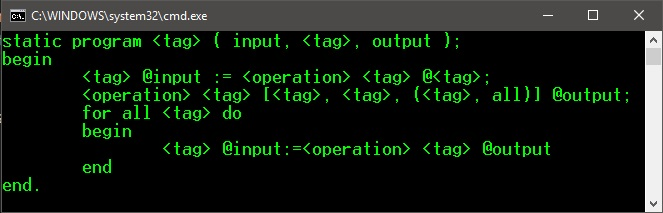
\includegraphics[scale=1]{test1}
\end{center}
Зеленый цвет означает то, что данная последовательность символов принадлежит грамматике.

Теперь внесем в данный тест ошибку (например, удалим "$<$"\ из середины цепочки). Результат будет следующим:\\


\begin{center}
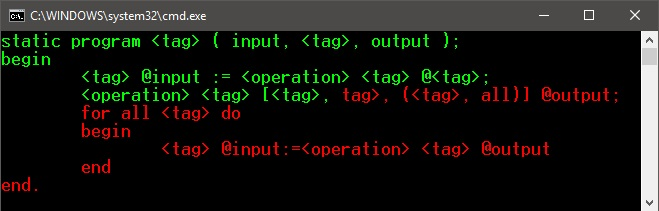
\includegraphics[scale=1]{test2}
\end{center}
Теперь половина цепочки подсвечена красным. Это значит, что на этой позиции распознаватель не смог перейти в какое-либо состояние, то есть зеленая часть является корректной, а в красной есть ошибка.
\\

Рассмотрим еще один вариант ошибки: что если распознаватель прочел всю цепочку, но так и не попал в конечное состояние? Для этого удалим завершающий символ "." из первого тестового примера:\\

\begin{center}
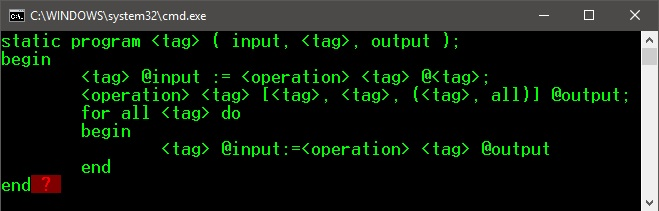
\includegraphics[scale=1]{test3}
\end{center}
Вся входная цепочка зеленая, однако в конце вывода присутствует красный вопросительный знак, который сигнализирует то, что цепочка закончилась, но конечное состояние достигнуто не было (т.е. возможно ввод не был прерван).


\end{document}
